\documentclass{article}

\usepackage[T1]{fontenc}

\usepackage{fancyhdr}
\usepackage{extramarks}
\usepackage{amsmath}
\usepackage{amsthm}
\usepackage{amsfonts}
\usepackage{tikz}
\usepackage{algorithm}
\usepackage{algpseudocode}
\usepackage{enumitem}

\usepackage[mono=false]{libertine}


\usetikzlibrary{automata,positioning}

%
% Basic Document Settings
%

\topmargin=-0.45in
\evensidemargin=0in
\oddsidemargin=0in
\textwidth=6.5in
\textheight=9.0in
\headsep=0.25in

\linespread{1.1}

\pagestyle{fancy}
\lhead{\hmwkAuthorName}
\chead{\hmwkClass: \hmwkTitle}
\rhead{\firstxmark}
\lfoot{\lastxmark}
\cfoot{\thepage}

\renewcommand\headrulewidth{0.4pt}
\renewcommand\footrulewidth{0.4pt}

\setlength\parindent{0pt}

%
% Create Problem Sections
%

\newcommand{\enterProblemHeader}[1]{
    \nobreak\extramarks{}{Problem \arabic{#1} continued on next page\ldots}\nobreak{}
    \nobreak\extramarks{Problem \arabic{#1} (continued)}{Problem \arabic{#1} continued on next page\ldots}\nobreak{}
}

\newcommand{\exitProblemHeader}[1]{
    \nobreak\extramarks{Problem \arabic{#1} (continued)}{Problem \arabic{#1} continued on next page\ldots}\nobreak{}
    \stepcounter{#1}
    \nobreak\extramarks{Problem \arabic{#1}}{}\nobreak{}
}

\setcounter{secnumdepth}{0}
\newcounter{partCounter}
\newcounter{homeworkProblemCounter}
\setcounter{homeworkProblemCounter}{1}
\nobreak\extramarks{Problem \arabic{homeworkProblemCounter}}{}\nobreak{}

%
% Homework Problem Environment
%
% This environment takes an optional argument. When given, it will adjust the
% problem counter. This is useful for when the problems given for your
% assignment aren't sequential. See the last 3 problems of this template for an
% example.
%
\newenvironment{homeworkProblem}[1][-1]{
    \ifnum#1>0
        \setcounter{homeworkProblemCounter}{#1}
    \fi
    \section{Problem \arabic{homeworkProblemCounter}}
    \setcounter{partCounter}{1}
    \enterProblemHeader{homeworkProblemCounter}
}{
    \exitProblemHeader{homeworkProblemCounter}
}

%
% Homework Details
%   - Title
%   - Due date
%   - Class
%   - Section/Time
%   - Instructor
%   - Author
%

\newcommand{\hmwkTitle}{Homework\ \#6}
\newcommand{\hmwkDueDate}{April 24, 2018}
\newcommand{\hmwkClass}{Design and Analysis of Algorithms}
\newcommand{\hmwkClassInstructor}{Professor Kasturi Varadarajan}
\newcommand{\hmwkAuthorName}{\textbf{Alic Szecsei}}

%
% Title Page
%

\title{
    \vspace{2in}
    \textmd{\textbf{\hmwkClass:\ \hmwkTitle}}\\
    \normalsize\vspace{0.1in}\small{Due\ in\ class\ on\ \hmwkDueDate}\\
    \vspace{0.1in}\large{\textit{\hmwkClassInstructor}}
    \vspace{3in}
}

\author{\hmwkAuthorName}
\date{}

\renewcommand{\part}[1]{\textbf{\large Part \Alph{partCounter}}\stepcounter{partCounter}\\}

%
% Various Helper Commands
%

% Useful for algorithms
\newcommand{\alg}[1]{\textsc{\bfseries \footnotesize #1}}

% For derivatives
\newcommand{\deriv}[1]{\frac{\mathrm{d}}{\mathrm{d}x} (#1)}

% For partial derivatives
\newcommand{\pderiv}[2]{\frac{\partial}{\partial #1} (#2)}

% Integral dx
\newcommand{\dx}{\mathrm{d}x}

% Alias for the Solution section header
\newcommand{\solution}{\textbf{\large Solution}}

% Probability commands: Expectation, Variance, Covariance, Bias
\newcommand{\E}{\mathrm{E}}
\newcommand{\Cov}{\mathrm{Cov}}
\newcommand{\Bias}{\mathrm{Bias}}

% Set from 1 to N
\newcommand{\XYZ}[1]{\left\{1,\ldots,{#1}\right\}}
\newcommand{\Break}{\textbf{break} }
\newcommand{\Var}[1]{\textsf{#1}}

\begin{document}

\maketitle

\pagebreak

\begin{homeworkProblem}

For any flow network $G$ and any vertices $u$ and $v$ let $bottleneck_G(u,v)$ denote the maximum, over all paths $\pi$ in $G$ from $u$ to $v$, of the minimum-capacity edge along $\pi$.

\begin{enumerate}[label=(\alph*)]
\item Describe and analyze an algorithm to compute $bottleneck_G(s,t)$ in $O(E \log V)$ time. 
\end{enumerate}

\solution\\

\part 

Solution

\end{homeworkProblem}

\pagebreak

\begin{homeworkProblem}

Suppose you have already computed a maximum flow $f*$ in a flow network $G$ with \emph{integer} edge capacities.

\begin{enumerate}[label=(\alph*)]
\item Describe and analyze an algorithm to update the maximum flow after the capacity of a single edge is increased by 1.
\item Describe and analyze an algorithm to update the maximum flow after the capacity of a single edge is decreased by 1.
\end{enumerate}

Both algorithms should be significantly faster than recomputing the maximum flow from scratch. \\

\solution\\

\part 

Solution

\part 

Solution

\end{homeworkProblem}

\pagebreak

\begin{homeworkProblem}

The Island of Sodor is home to a large number of towns and villages, connected by an extensive rail network. Recently, several cases of a deadly contagious disease (either swine flu or zombies; reports are unclear) have been reported in the village of Ffarquhar. The controller of the Sodor railway plans to close down certain railway stations to prevent the disease from spreading to Tidmouth, his home town. No trains can pass through a closed station. To minimize expense (and public notice), he wants to close down as few station as possible. However, he cannot close the Ffarquhar station, because that would expose him to the disease, and he cannot close the Tidmouth station, because then he couldn?t visit his favorite pub.\\

Describe and analyze an algorithm to find the minimum number of stations that must be closed to block all rail travel from Ffarquhar to Tidmouth. The Sodor rail network is represented by an undirected graph, with a vertex for each station and an edge for each rail connection between two stations. Two special vertices $f$ and $t$ represent the stations in Ffarquhar and Tidmouth.\\

For example, given the following input graph, your algorithm should return the number 2.

\begin{figure}[h]
	\centering
		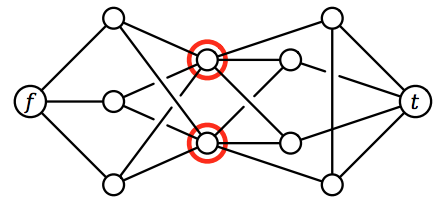
\includegraphics[scale=.75]{images/problem3}
\end{figure}

\solution\\

Solution

\end{homeworkProblem}

\pagebreak

\begin{homeworkProblem}

Suppose we are given an $n \times n$ square grid, some of whose squares are colored black and the rest white. Describe and analyze an algorithm to determine whether tokens can be placed on the grid so that

\begin{enumerate}
\item every token is on a white square;
\item every row of the grid contains exactly one token; and
\item every column of the grid contains exactly one token
\end{enumerate}

\begin{figure}[h]
	\centering
		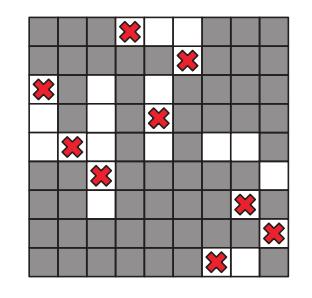
\includegraphics[scale=.75]{images/problem4}
\end{figure}

Your input is a two dimensional array $IsWhite$[1..$n$, 1..$n$] of booleans, indicated which squares are white. Your output is a single boolean. For example, given the grid above as input, your algorithm should return \alg{True}. \\

\solution\\

Solution

\end{homeworkProblem}

\pagebreak

\begin{homeworkProblem}

\emph{Ad-hoc} networks are made up of low-powered wireless devices. In principle, these networks can be used on battlefields, in regions that have recently suffered from natural disasters, and in other hard-to-reach areas. The idea is that a large collection of cheap, simple devices could be distributed through the area of interest (for example, by dropping them from an airplane); the devices would then automatically configure themselves into a functioning wireless network.\\

These devices can communicate only within a limited range. We assume all the devices are identical; there is a distance $D$ such that two devices can communicate if and only if the distance between them is at most $D$.\\

We would like our ad-hoc network to be reliable, but because the devices are cheap and low-powered, they frequently fail. If a device detects that it is likely to fail, it should transmit its information to some other $backup$ device within its communication range. We require each device $x$ to have $k$ potential backup devices, all within distance $D$ of $x$; we call
these $k$ devices the \textbf{\textit{backup set}} of x. Also, we do not want any device to be in the backup set of too many other devices; otherwise, a single failure might affect a large fraction of the network. \\

So suppose we are given the communication radius $D$, parameters $b$ and $k$, and an array $d$[1 .. $n$, 1 .. $n$] of distances, where $d[i, j]$ is the distance between device $i$ and device $j$. Describe an algorithm that either computes a backup set of size $k$ for each of the $n$ devices, such that no device appears in more than $b$ backup sets, or reports (correctly) that
no good collection of backup sets exists. \\

\solution\\

Solution

\end{homeworkProblem}

\end{document}